In this assignment, we are given measurements of air pollution (NO) gathered from a busy street in Copenhagen over a period of 24 hours. Since the measurements are taken hourly, we would like to fit a model (i.e.\ fit a smooth curve to the measurements) in order to compute the [NO] at any given point in time over the 0 to 24 hour interval. 

We assume that the data given represents the true signal plus the data errors. The latter captures errors in the measurement device (i.e.\ noise) as well as random variations inherent to the physical process that creates the data. In our case, the physical process is the "automobile-traffic system." 

Our data fitting goal is to create a parametric model that captures the behavior of this system, and which gives reliable estimates of the measured data (without being too sensitive to the data errors). We create the model by employing a least squares fit (LSQ) approach, which minimizes the sum of the squared residuals in order to find the best-fit model parameters.  

Under the LSQ approach, we make the following assumptions:

\begin{enumerate}[label={\bf Assumption~\arabic*},leftmargin=*]
\item The data and the errors are independent.

\item The data errors are "white noise", i.e.\ random and uncorrelated, have a mean of zero, have the same variance and are normal distributed.
\end{enumerate}
           
             
\subsection{Matlab Code}
We create a function (NOfit.m) that computes the Least Squares Fit of the data given. See Appendix~\ref{code:part1} for the function's code.   

\subsection{Testing the Software}
We test our matlab function for a model of order n = 3, which should not be a reliable model. We obtain the same residual norm of 292.558 as provided by the instructors. Figure~\ref{fig:figure1} below shows how the model approximates the observed data, and lists its solution coefficients ($x* = [186.806 -44.936 -93.429]$).

\begin{figure}[htb]
\centering
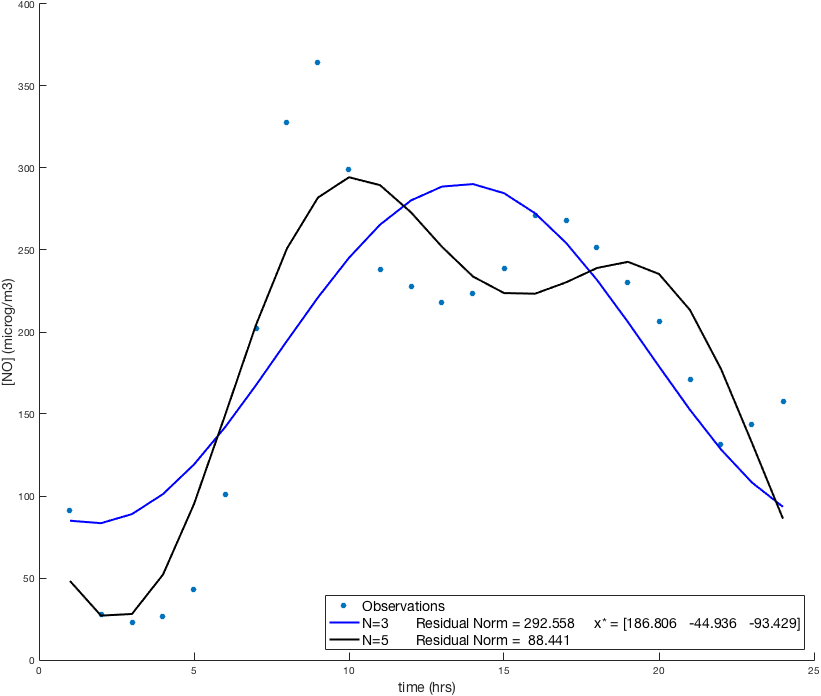
\includegraphics[width=0.7\textwidth]{../img/figure1}
\caption{LSQ Model fit for n = 3 (blue line) and n = 5 (black line). The figure shows how the model with 3 features fails to capture the bimodal structure of the observed data. The model with 5 features better captures the behavior, but still fails to provide good estimates of the observed data.}
\label{fig:figure1}
\end{figure}

\subsection{The Optimal Order of the Fit}
We want our model to capture the main behavior of the observed data, which consists of the pure data plus the data error (ideally, we would want our model to capture the pure-data function only). The residuals play an important role in evaluating how well the model does this. 

The residuals consist of two things: the data error ($e_i$) and the approximation error ($\Gamma(t_i) - M(x,t_i)$). 

\begin{equation}
r_{i} = e_{i} + (\Gamma(t_{i}) - M(x,t_{i}))
\label{eq:firstEquation}
\end{equation}


Because the data error and the approximation error have different statistical properties, and these properties carry over to the residuals, we can inspect the residuals to determine how well the model performs. 

We can not calculate the approximation errors because we do not have prior knowledge of the pure-data function. However, in the case where the approximation errors dominate the residuals, we would expect the residuals to behave more like the approximation errors. Generally speaking, the residuals will behave like a sampled signal (i.e. show trends and strong local correlations) and not like noise. 

\newpage
On the other hand, if data errors dominate the residuals, then we would expect the statistical properties of the data errors to carry over to the residuals. In that case, the residuals should behave more like white noise. As such, in our search for the best fit and optimal order n of that fit, we can analyze the residuals pertaining to each model and ask: 

\begin{enumerate}[label=\arabic*)]
\item Do the residuals behave like noise?
\item (Or alternatively) Do our residuals have strong, local correlations and/or trends?
\end{enumerate}

To answer these questions we perform a random signs test and an autocorrelation test.    

\begin{figure}[htbp]
\centering
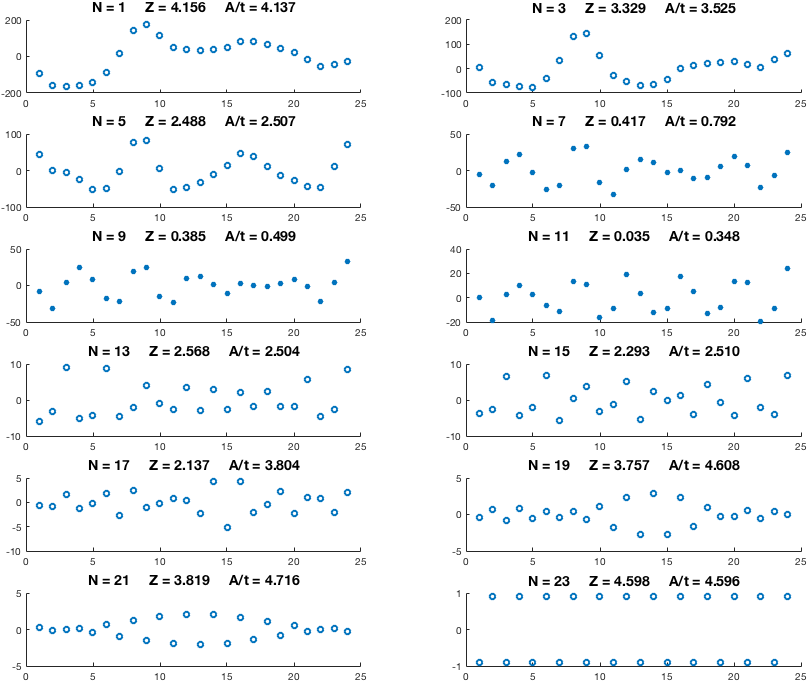
\includegraphics[width=0.9\textwidth]{../img/figure2}
\caption{The figures above show the residuals over time for each model of n'th order. The y-axis describes the magnitude of the residuals while the x-axis represents time in hours. Only the models of order 7, 9 and 11 (with filled blue bubbles) meet the criteria for randomness of signs and absence of trends.}
\label{fig:figure2}
\end{figure}


Figure~\ref{fig:figure2} shows the residuals as a function of time for models of different orders. The Z-Scores above each plot describe that the randomness of signs can be considered random at a 5 percent significance level if the Z-Score is less than 1.96. Only the models of order 7, 9 and 11 fit this criterion.

The autocorrelation over trend threshold ratio (A/T) is also shown for each model. Values greater than 1 indicate a trend is likely to be present in the residuals. Again, we observe that only the models of order 7, 9 and 11 fit this criterion. 

We can see in figure~\ref{fig:figure1} that when n is 3 and 5, the models fails to capture the behavior of the observed data, and hence we can conclude that the approximation errors are too large (bigger than the data errors). The residuals' tests support this. A visual inspection of figure~\ref{fig:figure2} shows obvious trends and the signs do not look random whatsoever. 

Models with n greater than 11 resemble the observed data the most (see figure~\ref{fig:figure4}), and have the smallest residuals (see table~\ref{tab:Table1}). However, while we want our model to capture the main behavior of the observed data as much as possible, we don't want the model that most resembles the observed data. Choosing a model based on having the smallest residuals endangers suffering from overfitting, where the model adapts to the data errors as well.

\begin{figure}[htbp]
\centering
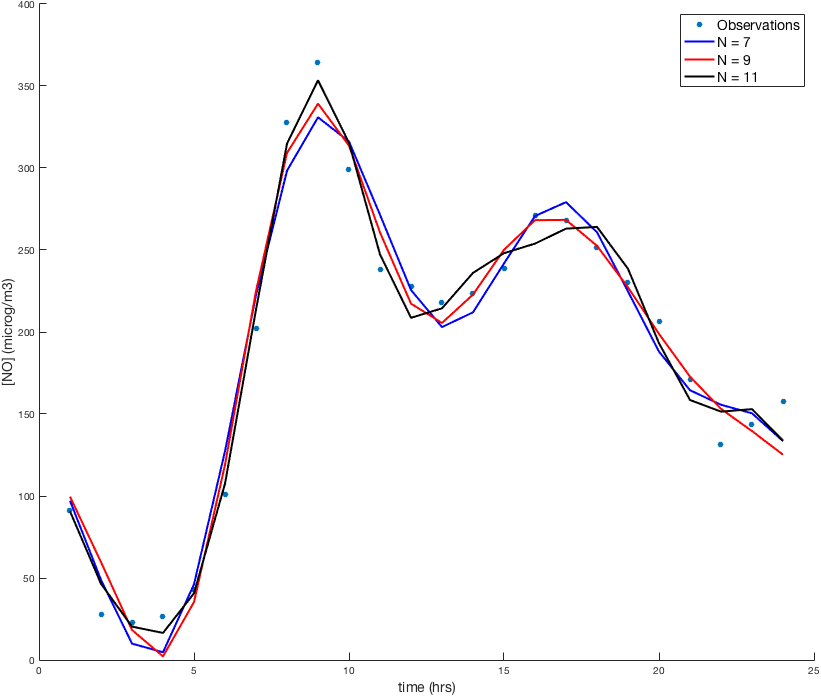
\includegraphics[width=0.7\textwidth]{../img/figure3}
\caption{LSQ model fit of n order 7, 9 and 11. The figure shows how these models capture the main behavior of the observed data without following it too closely. This leaves room for data error as opposed to adapting to the data error, which is undesirable.}
\label{fig:figure3}
\end{figure}


\begin{figure}[htbp]
\centering
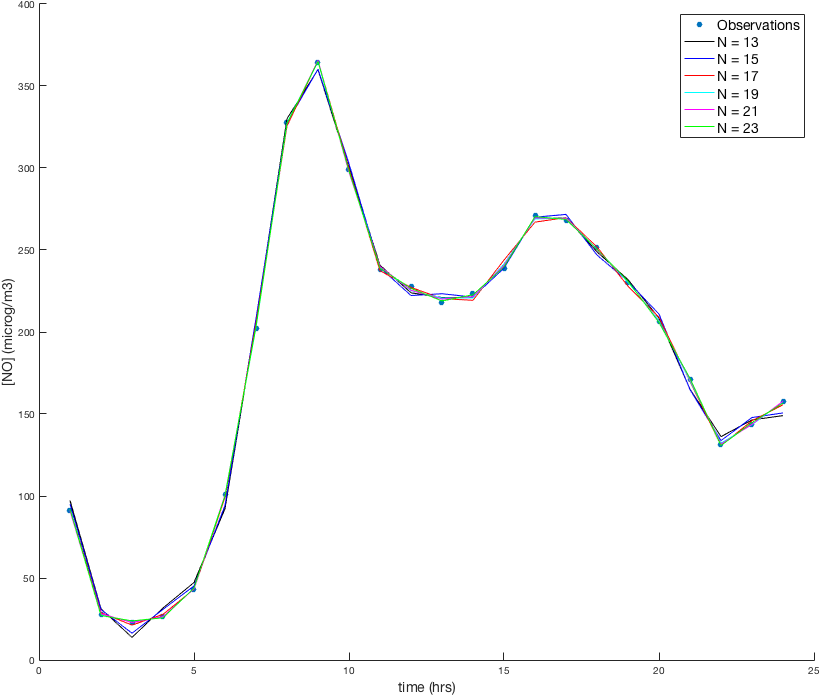
\includegraphics[width=0.7\textwidth]{../img/figure4}
\caption{LSQ model fit of n orders 13 to 23. The figure shows how these models follow the observed data too closely and risk adapting the behavior of the data error as well. This can result in overfitting.}
\label{fig:figure4}
\end{figure}

Indeed, for models n greater than 11, overfitting is a concern. They resemble the observed data too closely (see figure~\ref{fig:figure4}). The residuals do not look random either (save possibly for n = 15 albeit the test values say otherwise). 

Figure~\ref{fig:figure5} neatly captures this behavior. If we look at the scaled residual norms as a function of n, we should initially expect steep reductions as n increases since the model can better "match" the observed data with each increasing n. This steep decline embodies a diminishing approximation error. Afterwards, with larger n values, a plateu is reached and no longer the approximation error dominates the residuals, but rather the data error does. According to Chapter 2 of Least Squares Data Fitting with Applications, the transition between these two stages indicates the optimal choice for order n.  

\begin{figure}[htbp]
\centering
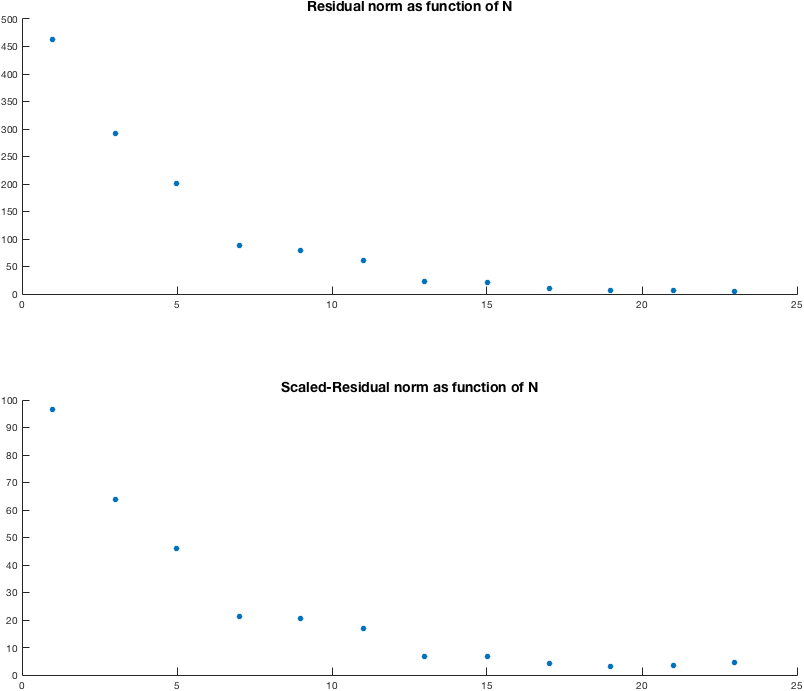
\includegraphics[width=0.7\textwidth]{../img/figure5}
\caption{The residual norm and its scaled version here are shown as a function of n. The figure shows how initially (for n = 1,3 and 5) the residuals (and the aproximation error) decrease rapidly as each additional n is able to fit a better model. After n = 7, the residuals flatten and the data error dominates the residuals. The transition between these two stages (from n =7 to n= 11) is an optimal zone for the order of the model.}
\label{fig:figure5}
\end{figure}
 
This transition in figure~\ref{fig:figure5} corresponds to n values of 7, 9 and 11, which coincide with the results of the residuals' tests. Given the arguments of approximation error dominance (for n = 3 and n = 5) and overfitting (for n = 13 and beyond), we conclude that 7, 9 and 11 are good candidates for optimal n order. Based on the residual tests, we choose model n order 11 as our optimal choice. 

\begin{table}[htbp]
\centering
\begin{tabular}{l|ccc}
\hline \hline 
\ $n$ & Residual Norm & Scaled Residual Norm \\ \hline
1 & 463.22	& 96.59 \\
3 & 292.56  & 63.84	 \\
5 & 201.15  & 46.15  \\
7 &  88.44  & 21.45  \\
9 &  79.27  & 20.47  \\
11 & 61.59	& 17.08 \\
13 & 22.19	& 6.69 \\
15 & 20.34	& 6.78 \\
17 & 10.78	& 4.07 \\
19 &  6.72  & 3.00 \\
21 &  6.00  & 3.47 \\
23 &  4.47  & 4.47 \\ 
\hline \hline
\end{tabular}
\caption{}
\label{tab:Table1}
\end{table} 

\newpage
\subsection{Estimating the Standard Deviation of the Solution Coefficients}
The scaled residual norm plays also another important role in assessing the uncertainty of our x* solution coefficients. In fact, if we assume that our residuals of our optimal n are dominated by data errors (as explained in section 1.3), then we can use the scaled residual norm as an estimate of the standard deviation of the noise (sigma). 

Section 1.3 and figure~\ref{fig:figure5} explain and depict respectively, that the transition between a diminishing approximation error and the plateu marks the area for an optimal n order, where the residuals are dominated by the data error. 

The sigma of the noise in turn, allows us to calculate the standard deviation of our x* solution coefficients with the following equation:

\begin{equation}
\mathrm{Cov}(x^{*}) = \zeta^{2}(A^{T}A)^{-1}
\end{equation}

Table~\ref{tab:Table2} lists the x* solution coefficients for model of n order 11 along with their respective standard deviations. 

\begin{table}[htbp]
\centering
\begin{tabular}{l|ccc}
\hline \hline 
$i$ & $x^*_{i}$ & Std. Deviation \\ \hline
1 & 186.81	& 3.49 \\
2 & -44.94  & 4.93	 \\
3 & -93.43  & 4.93  \\
4 & -60.89  & 4.93  \\
5 &  -7.28  & 4.93  \\
6 &  21.81	& 4.93 \\
7 &  47.37	& 4.93 \\
8 &   7.69	& 4.93 \\
9 &  -8.30	& 4.93 \\
10 &-11.54  & 4.93 \\
11 &  8.61  & 4.93 \\
\hline \hline
\end{tabular}
\caption{Table 2}
\label{tab:Table2}
\end{table}

\subsection{Concluding remarks}

By analyzing the residuals of the different models, we were able to choose an optimal one. Based on the assumptions of the LSQ fit approach, we knew that the statistical properties of the residuals should behave more like white noise (data error) as opposed to a sampled signal (approximation error). By performing a randomness of sings and an autocorrelation to trend threshold tests, we were able to evaluate the statistical properties of the residuals for each model. This guidance allowed us to pick an optimal model. In addition, the scaled residual norm for our optimal model served as an estimate for the standard deviation of the noise, which in turn allowed us to compute the covariance matrix of the solution coefficients (x*). This allowed us to approximate the standard deviation of each solution coefficient to get an understanding of the uncertainty involved in each coefficient. We can see from table 2 that this uncertainty becomes an issue for the 5th, 6th, and 8th to 11th coefficients. While a model of order n=7 provides as a whole coefficients with less uncertainty (the first seven on table 2), we ultimately opted for n=11 because the magnitude of the residual norm is significantly lower. If computational complexity was a concern, then model n=7 should provide a better alternative. However, with the given optimization task at hand, the computational demands of either of these models are not a concern, and model of n order 11 should provide better estimates to the observed data, yet without adapting to the data error.  